\begin{enumerate}
\item Univariate sparse quantile regression: \\
$$\min_{(\beta_0, \beta_1) \in \R^2}\frac{1}{n}\sum^n_{i = 1}\rho_\tau(y^{(i)} - \beta_0 -\beta_1 x^{(i)}) \text{ s.t. } \vert \beta_1\vert \leq t$$
\begin{enumerate}
\item Decompose unconstrained parameters into positive and negative part: $\beta_i = \beta^+_i - \beta^-_i \quad i = 0,1$ 
\item Transform absolute value: $\vert \beta_1\vert \leq t \iff \beta^+_1 + \beta^-_1 \leq t$
\item We can write $\rho_\tau(\underbrace{y^{(i)} - \beta_0 -\beta_1 x^{(i)}}_{=:r^{(i)}}) = \tau \cdot r^{(i)} \mathds{1}_{\{r^{(i)} > 0\}} - (1-\tau) \cdot r^{(i)} \mathds{1}_{\{r^{(i)} \leq 0\}} = \tau  \cdot {r^{(i)}}^+ + (1-\tau)\cdot {r^{(i)}}^-$
\item Transform equality of the residuals into two inequalities: \\
${r^{(i)}}^+ - {r^{(i)}}^- = y^{(i)} - \beta_0 -\beta_1 x^{(i)} \iff {r^{(i)}}^+ - {r^{(i)}}^- \leq y^{(i)} - \beta_0 -\beta_1 x^{(i)}$ and \\ 
$-{r^{(i)}}^+ + {r^{(i)}}^- \leq -y^{(i)} + \beta_0 +\beta_1 x^{(i)}$
\end{enumerate}
With this we get the standard form:\\
$\max_{\mathbf{z} \in \R^{4+2n}} \mathbf{c}^\top\mathbf{z}\quad $ s.t. $\mathbf{A}\mathbf{z} \leq \mathbf{b}$ and $\mathbf{z} \geq 0$ \\
with $\mathbf{z} = \begin{pmatrix}\beta_0^+\\ \beta_0^-\\ \beta_1^+\\ \beta_1^- \\ {r^{(1)}}^+ \\ \vdots \\ {r^{(n)}}^+ \\ {r^{(1)}}^- \\ \vdots \\ {r^{(n)}}^-  \end{pmatrix}, \mathbf{c} = \begin{pmatrix}0\\ 0\\ 0\\ 0 \\ -\tau \\ \vdots \\ -\tau \\ -(1-\tau) \\ \vdots \\ -(1-\tau)  \end{pmatrix},
\mathbf{A} = \begin{pmatrix}0 & 0 & 1 & 1 & 0 & \cdots  & 0 \\ 
\bm{1}_n & -\bm{1}_n & \mathbf{x} & -\mathbf{x} & \mathbf{I}_n && -\mathbf{I}_n \\ 
-\bm{1}_n & \bm{1}_n & -\mathbf{x} & \mathbf{x} & -\mathbf{I}_n && \mathbf{I}_n \
 \end{pmatrix},  \mathbf{b} = \begin{pmatrix}t\\ \mathbf{y}\\ -\mathbf{y} \end{pmatrix}$
 \item 
\begin{knitrout}
\definecolor{shadecolor}{rgb}{0.969, 0.969, 0.969}\color{fgcolor}\begin{kframe}
\begin{alltt}
\hlkwd{library}\hlstd{(ggplot2)}

\hlkwd{set.seed}\hlstd{(}\hlnum{123}\hlstd{)}
\hlstd{n} \hlkwb{=} \hlnum{30}
\hlstd{x} \hlkwb{=} \hlkwd{runif}\hlstd{(n)}
\hlstd{y} \hlkwb{=} \hlnum{2} \hlopt{*} \hlstd{x} \hlopt{+} \hlkwd{rgamma}\hlstd{(n,} \hlkwc{shape} \hlstd{=} \hlnum{1}\hlstd{)}

\hlstd{remp} \hlkwb{=} \hlkwa{function}\hlstd{(}\hlkwc{beta}\hlstd{)\{}
 \hlstd{r} \hlkwb{=} \hlstd{y} \hlopt{-} \hlstd{beta[}\hlnum{1}\hlstd{]} \hlopt{-} \hlstd{beta[}\hlnum{2}\hlstd{]} \hlopt{*} \hlstd{x}
 \hlkwd{return}\hlstd{(}\hlkwd{sum}\hlstd{(}\hlkwd{ifelse}\hlstd{(r} \hlopt{>} \hlnum{0}\hlstd{, tau}\hlopt{*}\hlstd{r,} \hlopt{-}\hlstd{(}\hlnum{1}\hlopt{-}\hlstd{tau)}\hlopt{*}\hlstd{r)))}
\hlstd{\}}

\hlstd{tau} \hlkwb{=} \hlnum{0.4}
\hlstd{tval} \hlkwb{=} \hlnum{1.7}

\hlstd{b} \hlkwb{=} \hlkwd{seq}\hlstd{(}\hlopt{-}\hlnum{3}\hlstd{,} \hlnum{3}\hlstd{,} \hlkwc{by}\hlstd{=}\hlnum{0.05}\hlstd{)}
\hlstd{bb} \hlkwb{=} \hlkwd{expand.grid}\hlstd{(}\hlkwc{X1} \hlstd{= b,} \hlkwc{X2} \hlstd{= b)}
\hlstd{fbb} \hlkwb{=} \hlkwd{apply}\hlstd{(bb,} \hlnum{1}\hlstd{,} \hlkwa{function}\hlstd{(}\hlkwc{beta}\hlstd{)} \hlkwd{remp}\hlstd{(beta))}

\hlstd{df} \hlkwb{=} \hlkwd{data.frame}\hlstd{(}\hlkwc{bb} \hlstd{= bb,} \hlkwc{fbb} \hlstd{= fbb)}
\hlstd{remp_plot} \hlkwb{=} \hlkwd{ggplot}\hlstd{()} \hlopt{+}
 \hlkwd{geom_contour_filled}\hlstd{(}\hlkwc{data} \hlstd{= df,} \hlkwd{aes}\hlstd{(}\hlkwc{x} \hlstd{= bb.X1,} \hlkwc{y} \hlstd{= bb.X2,} \hlkwc{z} \hlstd{= fbb))} \hlopt{+}
 \hlkwd{xlab}\hlstd{(}\hlkwd{expression}\hlstd{(beta[}\hlnum{0}\hlstd{]))} \hlopt{+}
 \hlkwd{ylab}\hlstd{(}\hlkwd{expression}\hlstd{(beta[}\hlnum{1}\hlstd{]))} \hlopt{+}
 \hlkwd{geom_hline}\hlstd{(}\hlkwc{yintercept} \hlstd{= tval,} \hlkwc{color}\hlstd{=}\hlstr{"red"}\hlstd{)} \hlopt{+}
 \hlkwd{geom_hline}\hlstd{(}\hlkwc{yintercept} \hlstd{=} \hlopt{-}\hlstd{tval,} \hlkwc{color}\hlstd{=}\hlstr{"red"}\hlstd{)}

\hlstd{remp_plot}
\end{alltt}
\end{kframe}
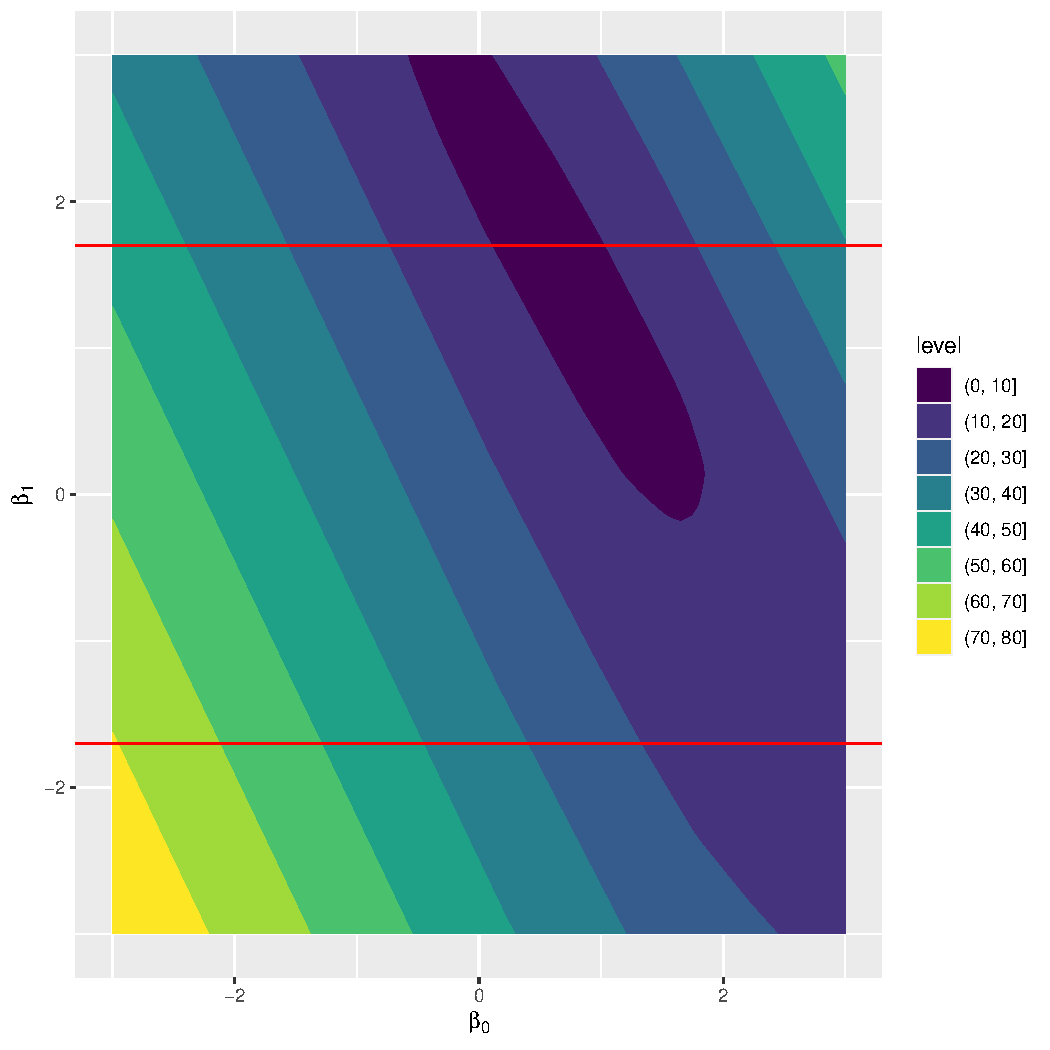
\includegraphics[width=0.5\linewidth]{figure/remp-plot-1} 
\end{knitrout}
\item 
\begin{knitrout}
\definecolor{shadecolor}{rgb}{0.969, 0.969, 0.969}\color{fgcolor}\begin{kframe}
\begin{alltt}
\hlkwd{library}\hlstd{(linprog)}
\end{alltt}


{\ttfamily\noindent\itshape\color{messagecolor}{\#\# Loading required package: lpSolve}}\begin{alltt}
\hlstd{Amat} \hlkwb{=} \hlkwd{c}\hlstd{(}\hlnum{0}\hlstd{,} \hlnum{0}\hlstd{,} \hlnum{1}\hlstd{,} \hlnum{1}\hlstd{,} \hlkwd{rep}\hlstd{(}\hlnum{0}\hlstd{,} \hlnum{2}\hlopt{*}\hlstd{n))}
\hlstd{Amat} \hlkwb{=} \hlkwd{rbind}\hlstd{(Amat,} \hlkwd{cbind}\hlstd{(}\hlnum{1}\hlstd{,} \hlopt{-}\hlnum{1}\hlstd{, x,} \hlopt{-}\hlstd{x,} \hlkwd{diag}\hlstd{(n),} \hlopt{-}\hlkwd{diag}\hlstd{(n)))}
\hlstd{Amat} \hlkwb{=} \hlkwd{rbind}\hlstd{(Amat,} \hlkwd{cbind}\hlstd{(}\hlopt{-}\hlnum{1}\hlstd{,} \hlnum{1}\hlstd{,} \hlopt{-}\hlstd{x, x,} \hlopt{-}\hlkwd{diag}\hlstd{(n),} \hlkwd{diag}\hlstd{(n)))}

\hlstd{bvec} \hlkwb{=} \hlkwd{c}\hlstd{(tval, y,} \hlopt{-}\hlstd{y)}
\hlstd{cvec} \hlkwb{=} \hlkwd{c}\hlstd{(}\hlnum{0}\hlstd{,} \hlnum{0}\hlstd{,} \hlnum{0}\hlstd{,} \hlnum{0}\hlstd{,} \hlkwd{rep}\hlstd{(tau, n),} \hlkwd{rep}\hlstd{(}\hlnum{1}\hlopt{-}\hlstd{tau, n))}

\hlstd{res} \hlkwb{=} \hlkwd{solveLP}\hlstd{(cvec, bvec, Amat,} \hlkwc{maximum} \hlstd{=} \hlnum{FALSE}\hlstd{,} \hlkwc{lpSolve} \hlstd{=} \hlnum{TRUE}\hlstd{)}

\hlstd{beta} \hlkwb{=} \hlkwd{c}\hlstd{(res}\hlopt{$}\hlstd{solution[}\hlnum{1}\hlstd{]} \hlopt{-} \hlstd{res}\hlopt{$}\hlstd{solution[}\hlnum{2}\hlstd{], res}\hlopt{$}\hlstd{solution[}\hlnum{3}\hlstd{]} \hlopt{-} \hlstd{res}\hlopt{$}\hlstd{solution[}\hlnum{4}\hlstd{])}

\hlkwd{ggplot}\hlstd{(}\hlkwd{data.frame}\hlstd{(}\hlkwc{x} \hlstd{= x,} \hlkwc{y} \hlstd{= y),} \hlkwd{aes}\hlstd{(}\hlkwc{x}\hlstd{=x,} \hlkwc{y}\hlstd{=y))} \hlopt{+}
 \hlkwd{geom_point}\hlstd{()} \hlopt{+}
 \hlkwd{geom_abline}\hlstd{(}\hlkwc{intercept} \hlstd{= beta[}\hlnum{1}\hlstd{],} \hlkwc{slope} \hlstd{= beta[}\hlnum{2}\hlstd{])}
\end{alltt}
\end{kframe}
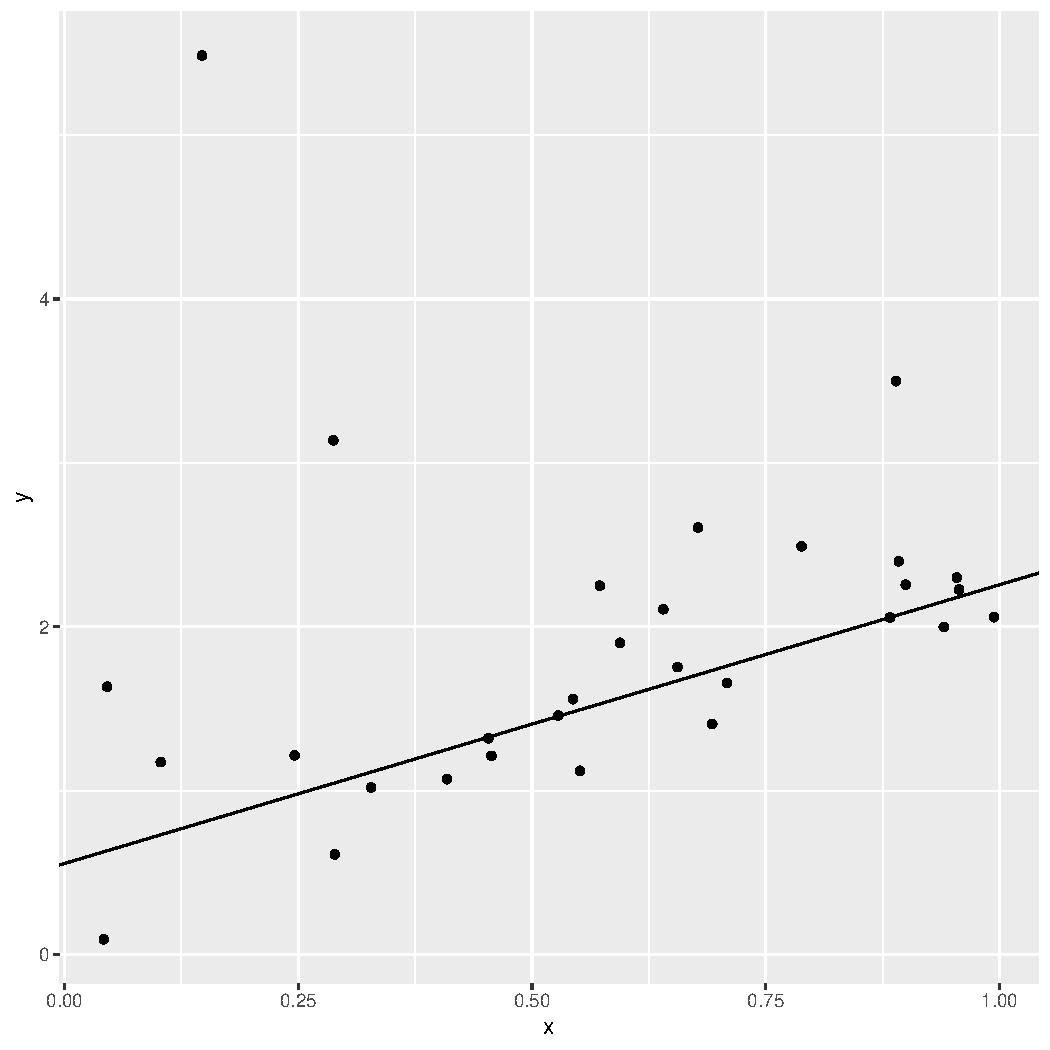
\includegraphics[width=0.5\linewidth]{figure/remp-lpsolve-1} 
\begin{kframe}\begin{alltt}
\hlstd{remp_plot} \hlopt{+}   \hlkwd{geom_point}\hlstd{(}\hlkwc{data}\hlstd{=}\hlkwd{data.frame}\hlstd{(}\hlkwc{x} \hlstd{= beta[}\hlnum{1}\hlstd{],} \hlkwc{y} \hlstd{= beta[}\hlnum{2}\hlstd{]),}
            \hlkwd{aes}\hlstd{(}\hlkwc{x}\hlstd{=x,} \hlkwc{y}\hlstd{=y),} \hlkwc{color}\hlstd{=}\hlstr{"lightblue"}\hlstd{)}
\end{alltt}
\end{kframe}
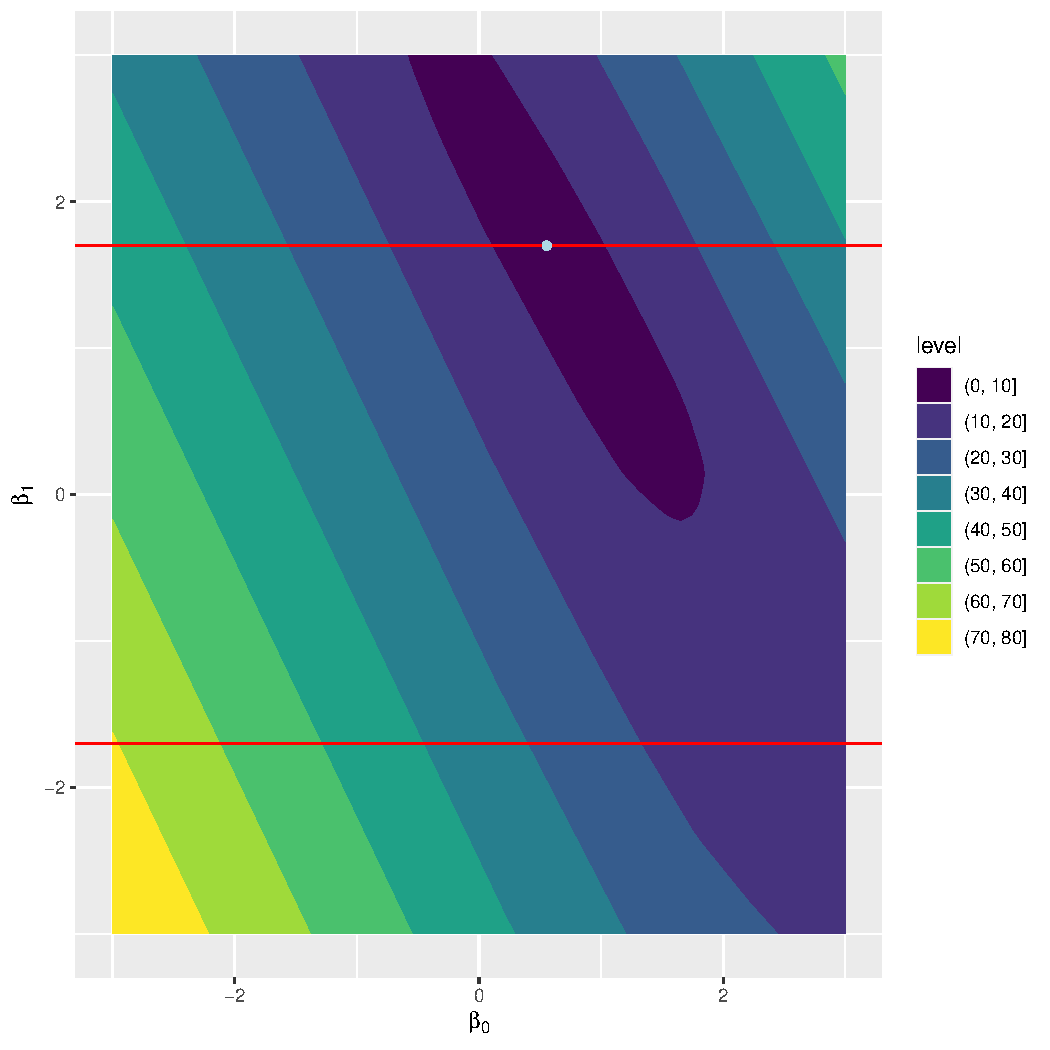
\includegraphics[width=0.5\linewidth]{figure/remp-lpsolve-2} 
\end{knitrout}
\item 
\end{enumerate}
